\documentclass{article}
\usepackage[T1]{fontenc}
\usepackage{lmodern}
\usepackage{graphicx}
\usepackage{amsmath,amssymb}
\usepackage[a4paper,margin=2cm]{geometry}
\usepackage[absolute,overlay]{textpos}
\setlength{\TPHorizModule}{1mm}
\setlength{\TPVertModule}{1mm}
\usepackage[indonesian]{babel}
\usepackage{hyperref}
\setlength{\emergencystretch}{2em}
% unit: Halaman 115

\begin{document}

% === Halaman 115 (python/native) ===

• Jerman sangat percaya diri bahwa Enigma tidak 

akan dapat dipecahkan.

• Namun, dengan bantuan Polandia,  Perancis 

dan Inggris kemudian membuat mesin pemecah 

Enigma baru ini, yang diberi nama bombe.

• Bombe dirancang oleh Alan Turing.

• Bombe berhasil memecahkan Enigma Cipher buatan Jerman.

• Keberhasilan memecahkan Enigma Cipher dianggap sebagai faktor yang 

memperpendek perang dunia kedua menjadi hanya dua tahun. 

Coba simulator online Enimga di: https://www.101computing.net/enigma/enigma-instructions.html 

115

% deskripsi: gambar native xref 412
\noindent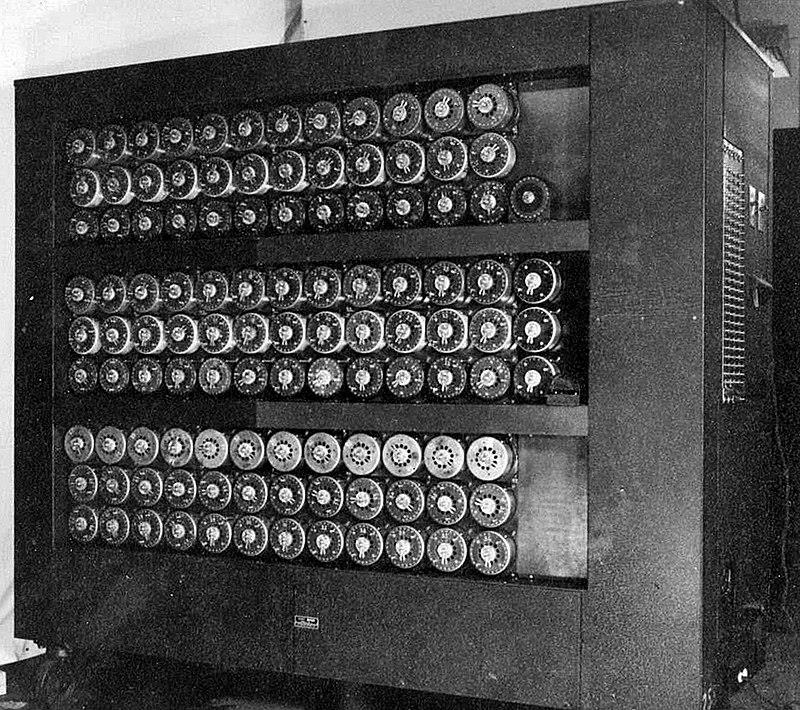
\includegraphics[width=0.85\textwidth]{../../images/python/page_115_img_01.jpeg}

\end{document}
